\section{Rozwiązania projektowe}

Niniejszy projekt tworzony jest dla klienta zewnętrznego, firmy zajmującej się
dystrybucją i sprzedażą rowerów. Stawiane przed deweloperami wymagania są zatem
podobne do tych, jakie są udziałem większości zespołów zajmujących się
implementacją rozwiązań internetowych. Celem projektu jest stworzenie
internetowego sklepu, który umożliwiałby zarówno kupowanie (zamawianie)
produktów związanych z szeroko pojętą branżą rowerową jak i śledzenie statusu
takich zamówień, zarządzanie nimi oraz ich ewentualne usuwanie. System powinien
także współpracować z pracownikami firmy Bike Shop sp. z.o.o. w zakresie obsługi
nowych dostaw, wprowadzania i zdobywania informacji o zamówieniach oraz kontaktów z
klientami. Działanie systemu można zatem podzielić na dwie główne kategorie:

\begin{description}
	\item[Moduł dla klientów] \hfill \\
	Składanie zamówień, edycja wprowadzonych danych na temat klientów, wydawanie
	opinii na temat sklepu, składanie zapytań
	\item[Moduł dla pracowników]
	Wprowadzanie danych o częściach rowerowych, odpowiadanie na zapytania klientów,
	informowanie o statusach zamówień, obsługa informatyczna dostaw
\end{description}

Oba opisane powyżej moduły koncentrują się przede wszystkim na częściach
rowerowych - to one są głównym powodem, dla którego tworzony jest projekt
informatyczny. Oznacza to, że pomimo pozornej rozróżnienia pomiędzy zadaniami,
jakie system ma spełniać dla użytkowników zewnętrznych (klientów) oraz
użytkowników wewnętrznych (pracowników) należy wymagania rozpatrywać całościowo,
bez podziału na osobne moduły. Zatem zarówno z punktu widzenia klienta jak i
zespołu zajmującego się projektowaniem i wdrażaniem implementacji nie istnieje
konieczność rozdziału funkcjonalności na 2 odrębne podsystemy. Istnieć może
tylko jeden system, dysponujący pełną funkcjonalnością. Poszczególne możliwości
dostępne będą tylko dla niektórych użytkowników, w zależności od ich roli w
systemie czy czasu, przez jaki korzystali ze sklepu (rabaty dla stałych
klientów itp.). Podejście takie niesie ze sobą szereg korzyści:

\begin{enumerate}
	\item Spójność tworzonego rozwiązania
	\item Analogiczne podejście do tworzonego oprogramowania
	\item Bardzo zbliżony interfejs graficzny
	\item Łatwość w zmianie ustawień dotyczących poszczególnych użytkowników (role)
	\item Łatwiejsza komunikacja pomiędzy klientami i pracownikami
	\item Brak konieczności tworzenia osobnych, bardzo podobnych implementacji
	\item Uspójnienie schematu - ułatwienie zarządzania
	\item Zwiększenie wydajności
\end{enumerate}

Jedynym potencjalnym problemem płynącym z jednolitej wersji systemu mogą być
ewentualne problemy z zapewnieniem bezpieczeństwa danych i uniemożliwienie
osobom niepowołanych dostęp do danych, które są przeznaczone tylko dla
specyficznych użytkowników. W czasie analizy należy zatem szczególnie zadbać o
tę część funkcjonalności, zarówno pod względem dostępu do danych w bazie danych
jak i inteferjsu graficznego (moduły dostępne tylko dla pracowników nie powinny
być widoczne dla klientów, prywatne dane klientów nie powinny z kolei być
dostępne dla nieupoważnionych pracowników).

\subsection{Architektura}

Jedną z głównych decyzji w czasie procesu projektowanie tworzonego systemu jest
wybór odpowiedniej architektury. Decyzja taka niesie za sobą szereg
konsekwencji, które mogą rzutować na poszczególne elementy decyzyjne, zmieniać
plany i kosztorysy całego projektu a także decydować o powodzeniu lub porażce
dla klienta. Nie bez znaczenia jest także element wydajnościowy, który w
przypadku sklepów internetowych jest jednym z kluczowych elementów całości,
decydującym nieraz o powodzeniu całego przedsięwzięcia.

W ostatnich latach zdecydowanie najpopularniejszym rozwiązaniem jest
architektura trójwarstwowa. Dzięki niej możliwe jest łatwe rozdzielenie
funkcjonalności na 3 główne części:
\begin{description}
	\item[Presentation Layer]
	\item[Business Layer]
	\item[Data Source]
\end{description}

\begin{figure}[h!]
    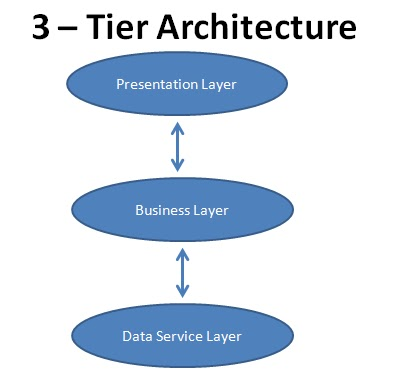
\includegraphics[width=\textwidth,
    height=0.5\textheight]{graphics/threetier.jpg}
  \caption{Ogólny schemat architektury projektowanego systemu}
\end{figure}

Każda z 3 części odpowiada za inną część związaną z procesowaniem i obsługą
zamówień:
\begin{description}
	\item[Presentation Layer] \hfill \\
		Moduł udostępniany na komputerze użytkownika, odpowiada za prezentowanie
		oferty sklepu, zbieranie akcji wykonywanych przez użytkownika i przekazywanie
		komunikacji do następnych warstw. Interfejs aplikacji
	\item[Business Layer] \hfill \\
		Moduł znajdujący się na serwerze aplikacyjnym, odpowiada za logikę całego
		systemu, koordynuje działania odpowiadające za zarządzanie zamówieniami.
		Przekazuje dane pomiędzy warstwami wyższą i niższą
	\item[Data Source] \hfill \\
		Odpowiada za trwałe przechowywanie danych a także udostępnia interfejs do ich
		pobierania, przetwarzania i zapisywania. Realizowana zazwyczaj za pomocą
		relacyjnych baz danych.
\end{description}

Dodatkowym modułem, niezbędnym w przypadku systemów, które będą wykorzystywane
przez kilkuset użytkowników jednocześnie (a taka jest docelowa przepustowość
serwerów projektowanego systemu), jest LoadBalancer, który jest odpowiedzialny
za rozkład obciążenia na osobne serwery realizujące te same funkcjonalności i
korzystające z tej samej bazy danych.

\begin{figure}[h!]
    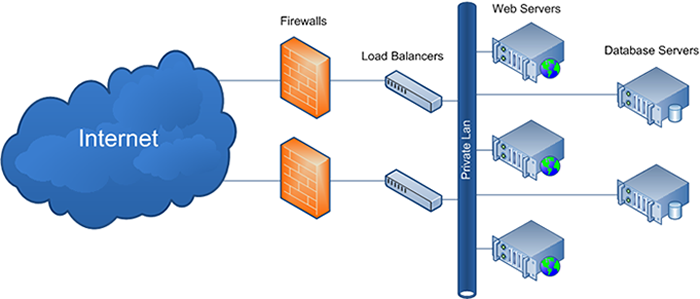
\includegraphics[width=\textwidth,
    height=0.5\textheight]{graphics/LoadBalancer.png}
  \caption{Schemat uwzględniający Load Balancer}
\end{figure}
Wybór architektury trójwarstwowej pociągnął za sobą także technologie, w których
zaimplementowane zostaną poszczególne warstwy. Z uwagi na dużą popularność, łatwość we wprowadzaniu zmian oraz wystarczająco rozbudowaną dokumentację zdecydowano się na wykorzystanie technologii JEE. Pozwala ona na stosunkowo łatwe i szybkie wdrażanie poszczególnych rozwiązań, ułatwia także zarządzanie już istniejącym projektem.

Ponieważ środowisko (zbiór technologii) Java Enterprise Edition jest bardzo
rozbudowane i posiada szereg różnych rozwiązań, konieczny stał się wybór tych
technologii, które w najlepszy sposób odwzierciedli i zapewni wsparcie dla
wymagań funkcjonalnych zdefiniowanych przez klienta. 

Zdecydowano się zatem na następujące rozwiązania technologiczne:

\begin{description}
\item[Frontend] \hfill \\
Ponieważ, jak wspomniano wcześniej, zdecydowano się na tworzenie systemu,
którego interfejs użytkownika zrealizowany jest w postaci aplikacji w
przeglądarce internetowej, wykorzystano technologie, związane z językiem Java,
które pozwalają na osadzenie w przeglądarce całej części wizualnej. W tym celu
wykorzystany zostanie wykorzystany język JavaScript wraz z technologiami HTML
oraz CSS. Pozwala to na otrzymanie wysokiej wydajności przy jednoczesnej
prostocie obsługi i implementacji. Dodatkowe funkcjonalności realizowane będą
także z wykorzystaniem biblioteki jQuery, która znacząco upraszcza proces
implementacji. Połączenie z pozostałymi warstwami obsługiwane jest z
wykorzystaniem protokołu HTTPS, co pozwala na zapewnienie bezpieczeństwa
(poprzez szyfrowanie) przekazywanych danych.
\item[Backend] \hfill \\
Jako serwer aplikacyjny zostanie wykorzystany IBM WebSphere, co pozwoli na
szybkie i łatwe implementowanie poszczególnych zależności pomiędzy modułami.
Każdy z modułów aplikacji obsługiwany jest przez zestaw Enterprise Java Beanów,
które zgromadzone są w kontenerze EJB. Komunikacja z bazą danych odbywa się z
wykorzystaniem technologii mapowania relacyjno-obiektowego zdefiniowanej w Java
Persistence API. Wybraną konkretną implementacją takiej technologii jest
framework Hibernate.
\item[Data Source] \hfill \\
Zdecydowano się na relacyjną bazę danych, które z powodzeniem są stosowane w
większości zastosowań w rozwiązaniach biznesowych i korporacyjnych od wielu lat.
Wybranym systemem bazodanowym jest Oracle w wersji 11.2. Jest to z jednej strony
najnowsza wersja systemu, pozwalająca na korzystanie z wielu obecnych tylko w
niej udogodnień a z drugiej jest to wersja stabilna, bez błędów i nieścisłości
obecnych w poprzednich edycjach wersji 11. Dane zapisywane są na zewnętrznych
macierzach dyskowych i duplikowane w celu zapewnienia bezpieczeństwa zapisu w
przypadku awarii.
\end{description}


\newpage
\begin{figure}[h!]
    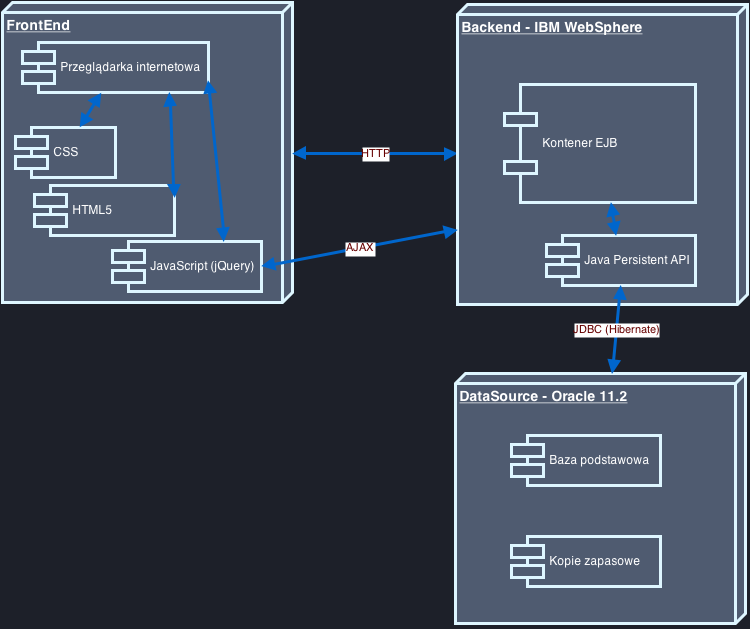
\includegraphics[width=\textwidth,
    height=0.5\textheight]{graphics/component.png}
  \caption{Architektura trójwarstwowa tworzonego systemu wraz z technologiami}
\end{figure}

Poszczegóły moduły komponentu EJB zaprezentowane są poniżej:
\begin{description}
  \item[Administracja] \hfill \\
  	Zarządzanie konfiguracją systemu, zapisem danych, umożliwienie przeglądania
  	logów
  \item[Logowanie] \hfill \\
  	Uwierzytelnianie użytkowników (klientów i pracowników) i ograniczanie lub
  	nadawanie uprawnień do poszczególnych elementów systemu
  \item[Klienci] \hfill \\
  	Obsługa informacji o klientach
  \item[Pracownicy] \hfill \\
    Obsługa informacji na temat pracowników
  \item[Części rowerowe] \hfill \\
  	Dane o częściach rowerowych, ich cenie, rozmiarze, dostępności
  \item[Zestawy rowerowe]
    Konfiguracja danych z modułu Części Rowerowe w zestawy, które mogą być
    sprzedawane całościowo
  \item[Zamówienia]
    Zarządzanie zamówieniami złożonymi przez klientów
  \item[Komunikacja klient-sklep]
    Obsługa powiadomień na temat zamówień, wymiany zapytań czy decyzji
    dotyczących zamówień
  \item[Komunikacja międzymodułowa]
    Obsługa pomiędzy pozostałymi modułami komponentu, zapis logów itp.
\end{description}


\begin{figure}[h!]
    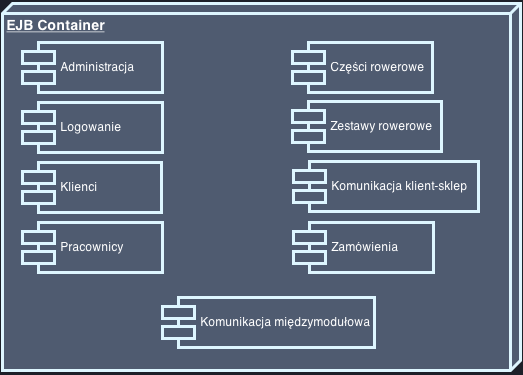
\includegraphics[width=\textwidth,
    height=0.5\textheight]{graphics/EJB.png}
  \caption{Widok szczegółowy kontenera EJB z podziałem na moduły}
\end{figure}
